% We import package amsmath before the documentclass to avoid the warning.
% Command '\usepackage{amsmath}' results in the following warning:
% Package amsmath Warning: Unable to redefine math accent \vec.
\RequirePackage{amsmath} % for environments such as align

\documentclass[runningheads]{llncs}

% If possible, figure files should be included in EPS format.

% If you use the hyperref package, please uncomment the following two lines
% to display URLs in blue roman font according to Springer's eBook style:
%\usepackage{color}
%\renewcommand\UrlFont{\color{blue}\rmfamily}

% The following code is used to remove the warning with subcaption package:
% ------------------------------
% Package caption Warning: Unknown document class (or package),
% standard defaults will be used.
% ------------------------------
% cf. https://teratail.com/questions/q2vuwf6skm5hph
\makeatletter
\def\caption@documentclass{elsarticle}
\makeatother

\usepackage{algorithm}
\usepackage{algpseudocode}
\usepackage{amssymb} % for \mathbb
\usepackage{array} % for m column type
\usepackage{bbm} % for \mathbbm
\usepackage{booktabs} % for \toprule, \midrule, \bottomrule
\usepackage{cleveref} % for \cref
\usepackage{csvsimple} % for \csvreader
\usepackage[T1]{fontenc} % for T1 font encoding
\usepackage{graphicx} % for \includegraphics
\usepackage{pgffor} % for \foreach
\usepackage[labelformat=simple]{subcaption} % for subfigure environment

% The following code is used to remove the warning with bibliography:
% ------------------------------
% Underfull \hbox (badness 2653) in paragraph at lines 28--34
% ------------------------------
% cf. https://tex.stackexchange.com/questions/10924/underfull-hbox-in-bibliography
\apptocmd{\sloppy}{\hbadness 10000\relax}{}{}


% set the path for figures
\graphicspath{{./data/}{./python/data/}}

% set the label format for subcaption
\renewcommand\thesubfigure{(\alph{subfigure})}

% settings for cleveref
\crefname{figure}{Fig.}{Figs.}
\crefname{table}{Table.}{Tables.}

% import the TeX file containing macro definitions
\newcommand{\ispace}{\mathbb{D}^{m}}
\newcommand{\Prec}{\operatorname{acc}}
\newcommand{\Cov}{\operatorname{cov}}
\newcommand{\cands}{\bar{\mathcal{A}}}
\algnewcommand{\IIf}[1]{\State\algorithmicif\ #1\ \algorithmicthen\ }
\renewcommand{\algorithmicrequire}{\textbf{Input:}}
\renewcommand{\algorithmicensure}{\textbf{Output:}}


\begin{document}

% Authentic title
\title{%
  R-LIME: Rectangular Constraints and Optimization for Local Interpretable
  Model-agnostic Explanation Methods}

% Abbreviated title for the running head
\titlerunning{%
  R-LIME: Rectangular Constraints and Optimization for LIME Methods
}

% Author names and ORCID IDs
\author{Genji Ohara\inst{1}\orcidID{0009-0000-5854-2820} \and
  Keigo Kimura\inst{1}\orcidID{0000-0002-3614-6568} \and
  Mineichi Kudo\inst{1}\orcidID{0000-0003-1013-3870}
}

% Abbreviated author list for the running head (First names are abbreviated)
% If there are more than two authors, 'et al.' is used.
\authorrunning{G. Ohara et al.}

% The authors' affiliations
\institute{Division of Computer Science and Information Technology\\
  Graduate School of Information Sci.\ and Tech.,
  Hokkaido University\\
  Sapporo 060-0814, JAPAN,\\
  \email{\{genji-ohara, kimura5, mine\}@ist.hokudai.ac.jp}}

% typeset the header of the contribution
\maketitle              %

% The abstract should briefly summarize the contents of the paper in
% 150--250 words.
\begin{abstract}
  In recent years, complex machine learning models such as deep neural networks
  have been used in various industrial fields due to their high accuracy.
  However, its complexity has been a major obstacle to implementation
  in decision-making situations where transparency of the decision process is required.
  In order to address this problem,
  various post-hoc explanation methods have been proposed,
  but they have not been able to achieve interpretability of
  both the explanation and its scope.
  We propose a new method, R-LIME,
  which interprets complex classifiers in an interpretable scope.
  R-LIME locally approximizes a complex decision boundary linearly
  in a rectangular region
  and maximizes the region as long as the accuracy of the linear
  classifier is higher than a specified threshold.
  The resulting rectangular region is interpretable for users because it is
  expressed as a conjunction of feature predicates.
  We demonstrate the effectiveness of the proposed method through qualitative
  and quantitative experiments using a real-world dataset.
  Finally, we discuss limitations and future work of the proposed method.
  % 148 words
  \keywords{Interpretable machine learning \and Local surrogate model}
\end{abstract}

\section{Introduction}
Machine learning models, such as deep learning and random forests,
have been widely employed in various industrial applications
due to their significant improvement in accuracy in recent years.
However,
the increasing complexity and black-box nature of these models pose challenges,
particularly in critical decision-making scenarios like healthcare and finance,
where the opacity of decision rationale becomes a major obstacle to
implementation.
Consequently,
there has been extensive research in the field of post hoc explanations
for machine learning models \cite{%
  ribeiro2016why,ribeiro2018anchors,radulovic2023bella,guidotti2018local}.

Existing methods on post hoc explanations categorize into
\emph{model-dependent} and \emph{model-agnostic} methods,
based on their dependence on the model's structure.
Model-dependent methods primarily focus on deep neural networks and
explain the models' behavior using their parameters.
While they allow a direct approach to the model,
applying the same method to models with different structures is often challenging.
On the other hand,
model-agnostic methods do not rely on the models' parameters and utilize only their output.
Although they are applicable to any model, available information is limited.
Model-agnostic methods further classify into
\emph{global} and \emph{local} methods based on their locality in input space.
Global methods aim to explain the model's behavior across the entire input space,
seeking explanations valid for any input.
However, providing global explanations becomes challenging as the model's complexity increases.
Local methods, in contrast, explain the model's output for a specific input
(focal point) in the vicinity of that input.
While local methods offer more simple and accurate explanations than global methods,
the scope of the explanation is limited to the vicinity of the focus point.

This paper specifically focuses on \emph{local} \emph{model-agnostic} methods.
For instance, LIME (Local Interpretable Model-agnostic Explanations)
\cite{ribeiro2016why} approximates the complex model's decision boundary
locally using a simpler model.
Although LIME enables users to interpret the local behavior of complex models,
it does not optimize the approximation region \cite{radulovic2023bella} and
the effective scope of the explanation is not explicitly presented
\cite{ribeiro2018anchors}.

To address the limitations of LIME,
we propose a new method called R-LIME (Ruled LIME),
which interprets complex classifiers in an interpretable region.
R-LIME locally approximates a complex decision boundary linearly
in a rectangular region and maximizes the region as long as the accuracy of the linear
classifier is higher than a specified threshold.
The resulting rectangular region is interpretable for users because it is
expressed as a conjunction of feature predicates.

\section{Related Work}
\begin{figure}[t]
  \centering
  \vspace{0.5cm}
  \begin{subfigure}[t]{0.55\textwidth}
    \centering
    
\includegraphics[width=\textwidth]{lime_vs_anchor_exp_a.png}
    \caption{Instances around the focal point.}\label{fig:lime_vs_anchor_exp_a}
    \vspace{0.5cm}
  \end{subfigure}
  \begin{subfigure}[t]{0.45\textwidth}
    \centering
    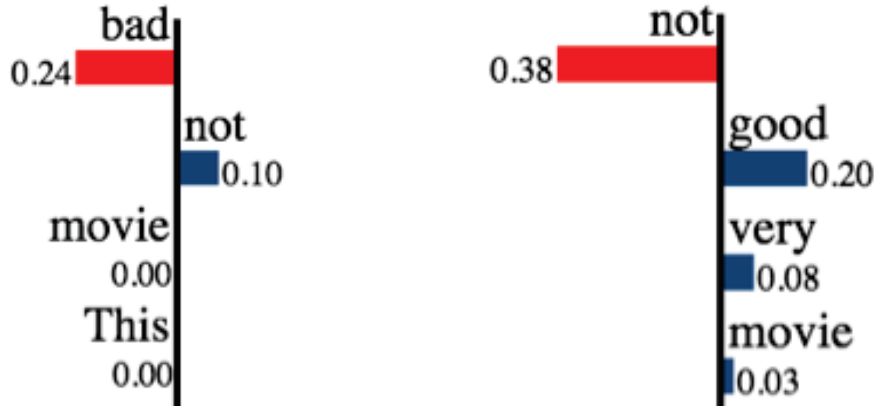
\includegraphics[width=\textwidth]{lime_vs_anchor_exp_b.png}
    \caption{%
      Explanations by LIME.
      They provide contributions of each feature to the output,
      but do not explicitly indicate its scope.
    }\label{fig:lime_vs_anchor_exp_b}
    \vspace{0.5cm}
  \end{subfigure}
  \begin{subfigure}[t]{0.55\textwidth}
    \centering
    
\includegraphics[width=\textwidth]{lime_vs_anchor_exp_c.png}
    \caption{%
      Explanations by Anchor.
      They provide the effective scope of the explanation,
      but do not provide details about the influence of each feature.
    }\label{fig:lime_vs_anchor_exp_c}
  \end{subfigure}
  \caption{%
    Explanations by LIME and Anchor
    for an LSTM sentiment prediction model \cite{ribeiro2018anchors}.
  }\label{fig:lime_vs_anchor_exp}
\end{figure}
In this chapter,
we provide an overview of existing research on local model-agnostic explanations,
particularly focusing on studies closely related to our proposed method.

\subsection{LIME (Local Interpretable Model-agnostic Explanations) \cite{ribeiro2016why}}
LIME locally
approximates a trained black-box classifier $f: \mathbb{R}^d \to \{0,1\}$
around a focal point $x \in \mathbb{R}^d$
by a linear classifier $g: \mathbb{R}^d \to \{0,1\}$
(\cref{fig:lime}).
The process involves:
\begin{enumerate}
  \item Obtaining a set of perturbed samples $\mathcal{Z}_p$ around $x$
        and the set of pseudo-labels $f(\mathcal{Z}_p) = \{f(z) \mid z \in \mathcal{Z}_p\}$.
  \item Learning a linear classifier $g$
        using $\mathcal{Z}_p$ and $f(\mathcal{Z}_p)$
        by minimizing the following loss function:
        \begin{equation}
          \label{eq:lime_loss}
          \mathcal{L}(f,g,\pi_x)=\sum_{z\in\mathcal{Z}_p}
          \pi_x(z){\left(f(z)-g(z)\right)}^2,
        \end{equation}
        where $\pi_x(z)$ is a weight function designed to be larger for samples
        closer to $x$, typically implemented using an exponential kernel.
\end{enumerate}

LIME provides valuable insights into the local behavior of the model
by showing the contribution of each feature to the output $f(x)$.
However, due to not explicitly indicating the perturbation region,
users cannot assess the effective scope of the explanation
\cite{ribeiro2018anchors}.
An example of explanation by LIME for an LSTM sentiment prediction model
is illustrated in \cref{fig:lime_vs_anchor_exp_b}.
The left explanation suggests that
the word "not" contributes to the model's positive prediction,
which does not apply to the instance on the right.
However, without the explicit perturbation region,
users might mistakenly apply the left explanation to the right instance,
potentially leading to a misunderstanding of the black-box model's behavior
\cite{ribeiro2018anchors}.

\subsection{Anchor \cite{ribeiro2018anchors}}\label{sec:anchor}
Anchor represents a rectangular region containing the focal point $x$,
expressed as a conjunction of feature predicates (a rule),
that maximizes the probability of the black-box classifier $f$
outputting $f(x)$ within the region.
It aims to highlight important features
contributing significantly to the output (\cref{fig:anchor}).

For a discrete $m$-dimensional input space $\ispace$
with a trained black-box classifier $f: \ispace \to \{0,1\}$,
an instance $x \in \ispace$, 
and a distribution $\mathcal{D}$ over the input space,
a rule $A(z) = a_{i_1}(z) \wedge a_{i_2}(z) \wedge \dots \wedge a_{i_t}(z)$ is defined.
The predicates $a_i(z)$ evaluate to true ($=1$) when $z_i = x_i$ and false ($=0$) otherwise.
The accuracy $\Prec(A)$ and coverage $\Cov(A)$ of the rule $A$ are defined as follows:
\begin{align}
  \Prec(A) & =\mathbb{E}_{z\sim\mathcal{D}(z|A)}
  [\mathbbm{1}_{f(z)=f(x)}], \label{eq:anchor_def_prec} \\
  \Cov(A)  & =\mathbb{E}_{z\sim\mathcal{D}(z)}[A(z)].
\end{align}

where $\mathcal{D}(z|A)$ is the conditional distribution in the region
where the rule $A$ returns true.
$\Prec(A)$ represents the probability that the output of $f$ matches
between the perturbation $z\sim\mathcal{D}(z|A)$ and the focal point $x$,
and $\Cov(A)$ expresses the probability that the perturbation $z$ fits into $A$.

Anchor maximizes coverage under the constraint that
the accuracy of the rule $A$ exceeds a given threshold $\tau$.
However, \cref{eq:anchor_def_prec} is not directly computable.
Introducing a confidence level $1-\delta$ $(0\le\delta\le1)$,
the accuracy constraint is relaxed as follows:
\begin{equation}
  \label{eq:const_prec}
  P(\Prec(A)\ge\tau)\ge1-\delta.
\end{equation}
Thus, the following optimization problem is solved:
\begin{equation}
  \label{eq:main_problem}
  A^*=\underset{A \text{~s.t. } P(\Prec(A)\ge\tau)\ge1-\delta\wedge A(x)=1}
  {\arg\max}\Cov(A).
\end{equation}

While Anchor provides an effective scope of the explanation,
the information it includes is less than LIME,
limiting its utility \cite{ribeiro2018anchors}.
An example of Anchor explanation for an LSTM sentiment prediction model
is depicted in \cref{fig:lime_vs_anchor_exp_c}.
The left explanation suggests that changing words other than "not" and "bad"
has little impact on the classifier's output.
While it clearly does not apply to the right instance,
the explanation does not provide details about the influence of each word,
resulting in less user insight into the model's behavior compared to LIME
(\cref{fig:lime_vs_anchor_exp_b}).

\subsection{%
  BELLA (Black box model Explanations by Local Linear Approximations)
  \cite{radulovic2023bella}
}
BELLA addresses the non-optimization of the approximation region,
a drawback of LIME,
by learning a local linear classifier $g$
using a subset $Z'$ of the dataset $Z$
instead of perturbed samples (\cref{fig:bella}).
The process involves:
\begin{enumerate}
  \item Computing the distance $d_x(z)$ for all instances $z$ in $Z$
        with respect to the focal point $x$.
  \item Selecting the $k$ instances with the smallest $d_x(z)$,
        forming a subset $Z_s(k) \subseteq Z$.
  \item Learning the local linear classifier $g$ using $Z_s(k)$
        and calculating the similarity measure $\mathcal{R}(k)$ between $f$ and $g$
        over $k=1,2,\dots,|Z|$.
  \item Obtaining the optimal $k^*$ by maximizing $\mathcal{R}(k)$.
\end{enumerate}

BELLA aims to enhance the reliability of explanations
by optimizing the approximation region for high-accuracy linear approximations.
However, it assumes direct access to the dataset $Z$ used for training the classifier,
making it inapplicable in scenarios where direct access to the dataset is restricted.
Additionally,
as BELLA presents the approximation region as a subset of the dataset,
its interpretability is lower compared to Anchor.

\section{Proposed Method}
\begin{figure}[tb]
  \centering
  \begin{subfigure}[t]{0.45\textwidth}
    \centering
    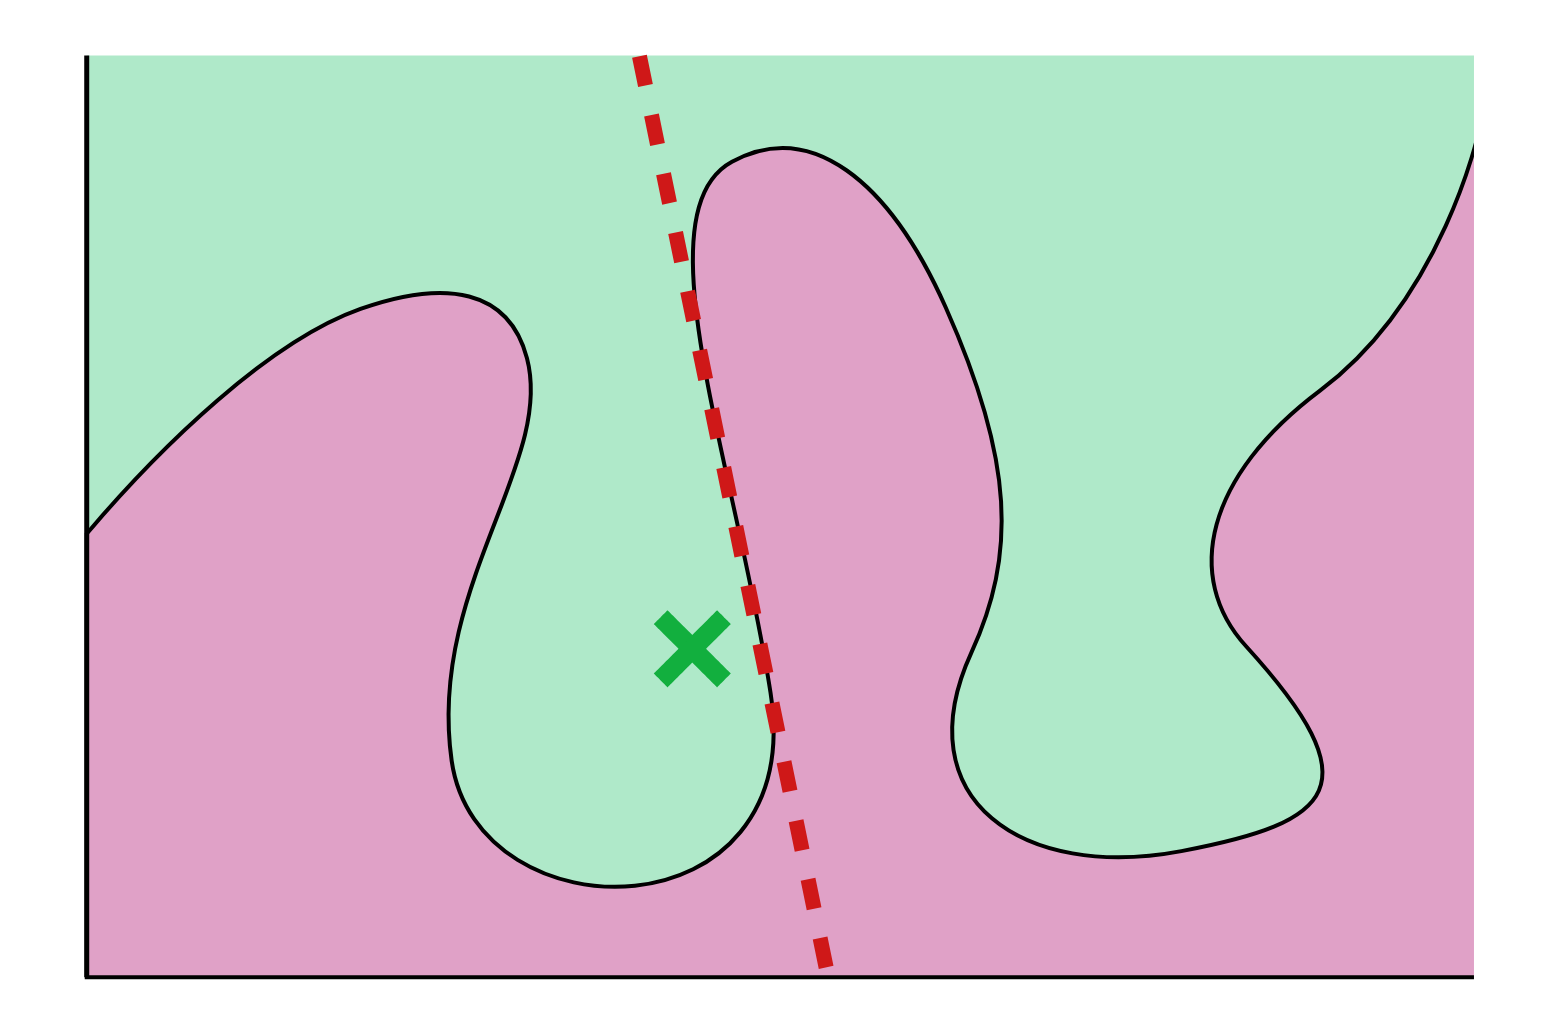
\includegraphics[width=\textwidth]{lime}
    \caption{%
      LIME: Locally approximates the decision boundary around the focal point.
    }\label{fig:lime}
  \end{subfigure}%
  \hfill
  \begin{subfigure}[t]{0.45\textwidth}
    \centering
    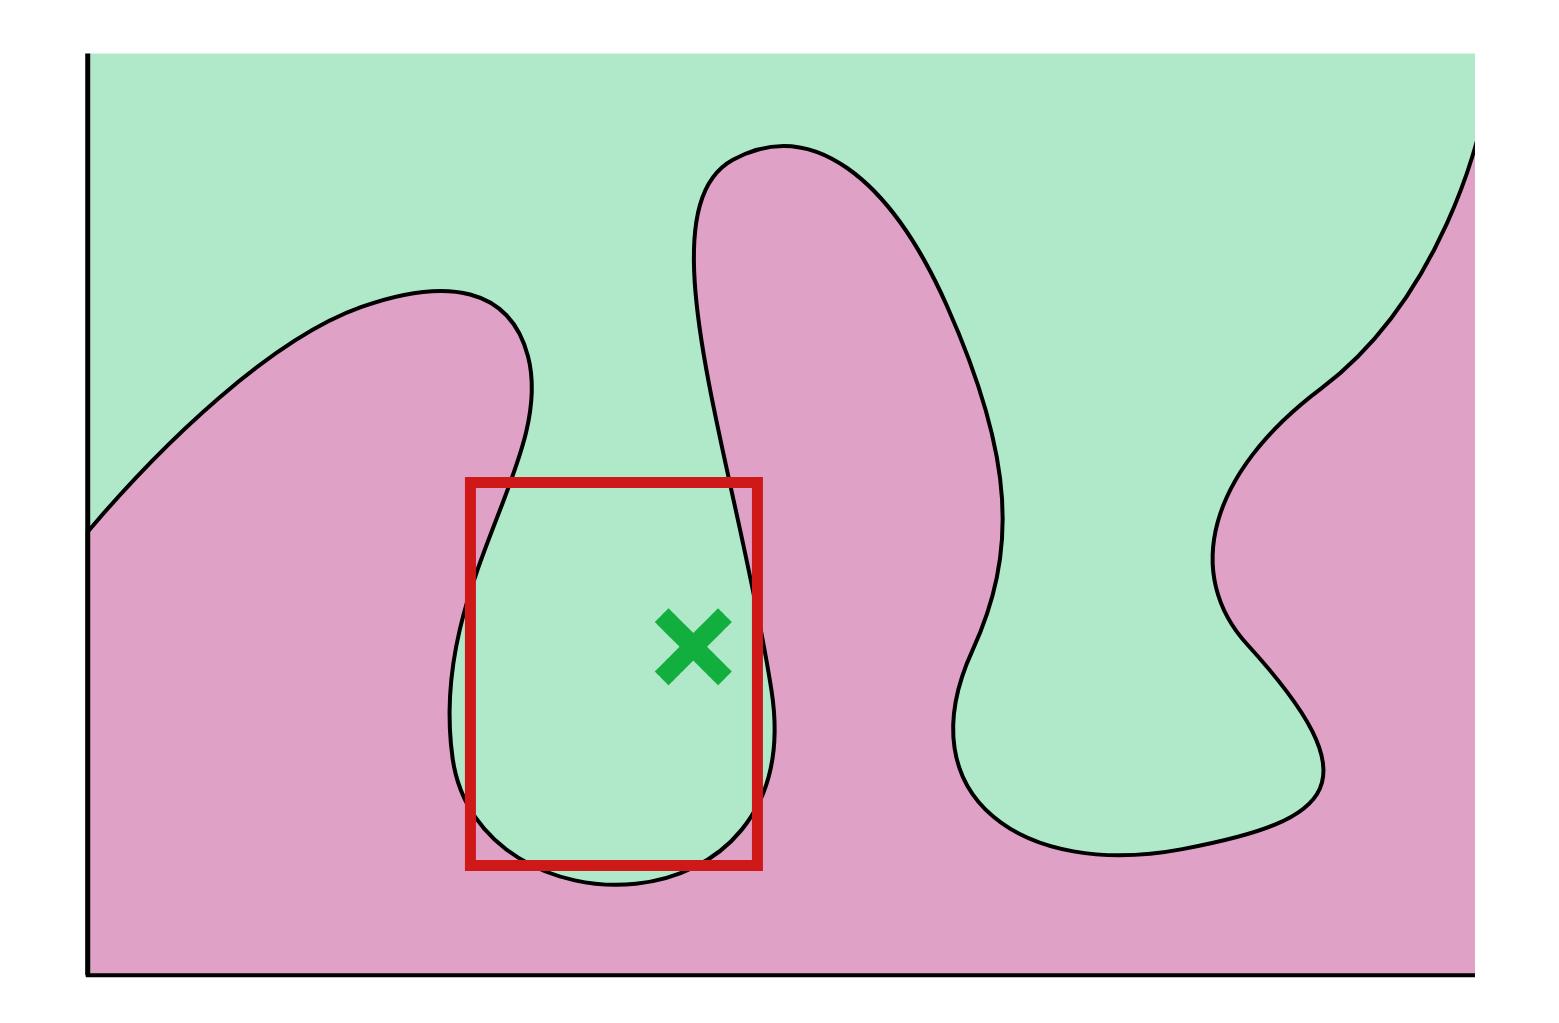
\includegraphics[width=\textwidth]{anchor}
    \caption{%
      Anchor: Maximizes coverage of a rectangular region
      containing the focal point under accuracy constraints.
    }\label{fig:anchor}
  \end{subfigure}
  \hfill
  \begin{subfigure}[t]{0.45\textwidth}
    \centering
    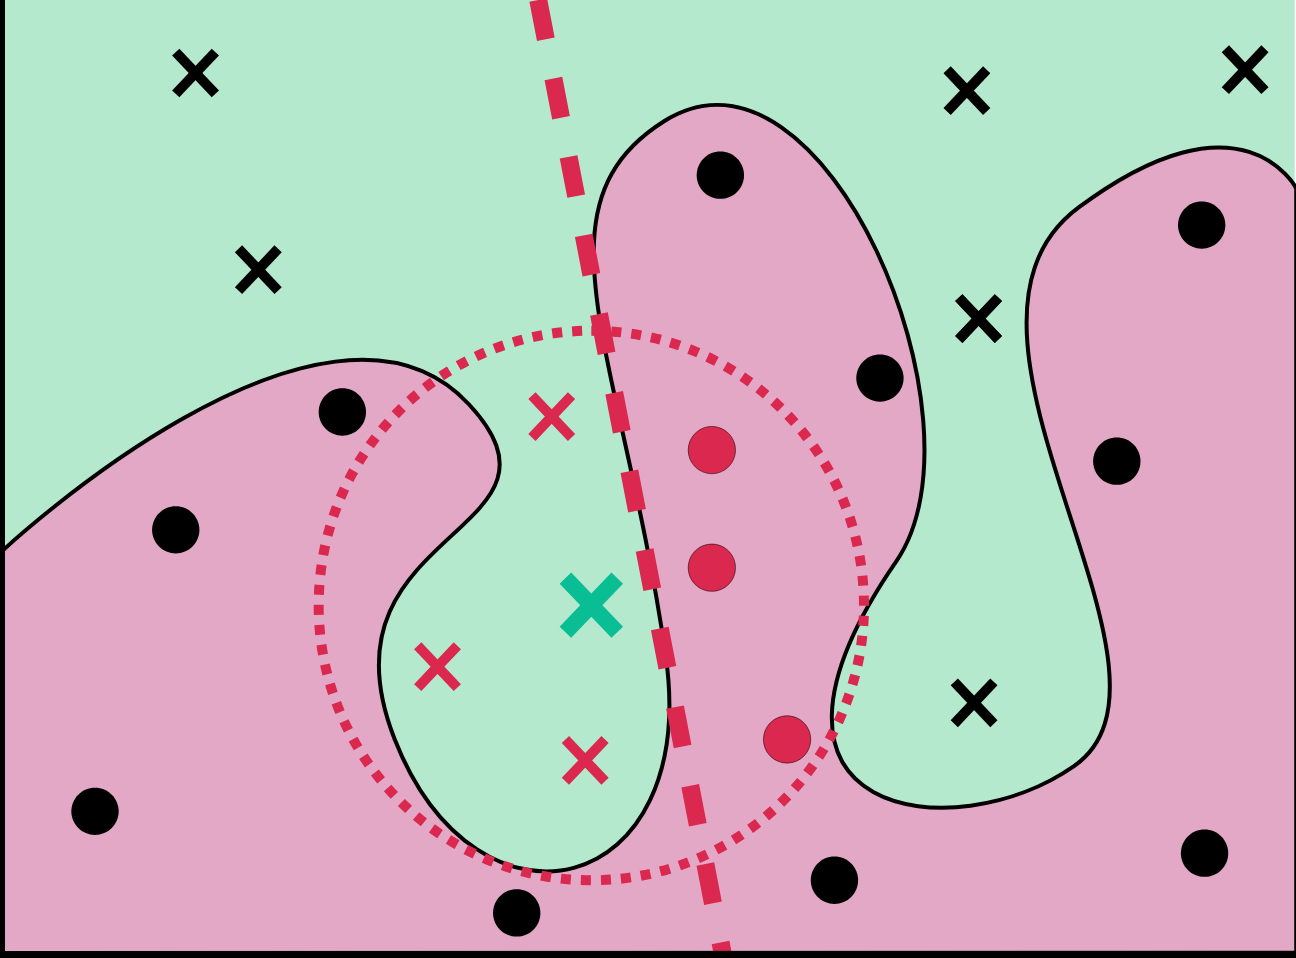
\includegraphics[width=0.85\textwidth]{bella}
    \caption{%
      BELLA: Explores a subset of the dataset,
      maximizing similarity between the local linear classifier
      and the black-box classifier.
    }\label{fig:bella}
  \end{subfigure}
  \hfill
  \begin{subfigure}[t]{0.45\textwidth}
    \centering
    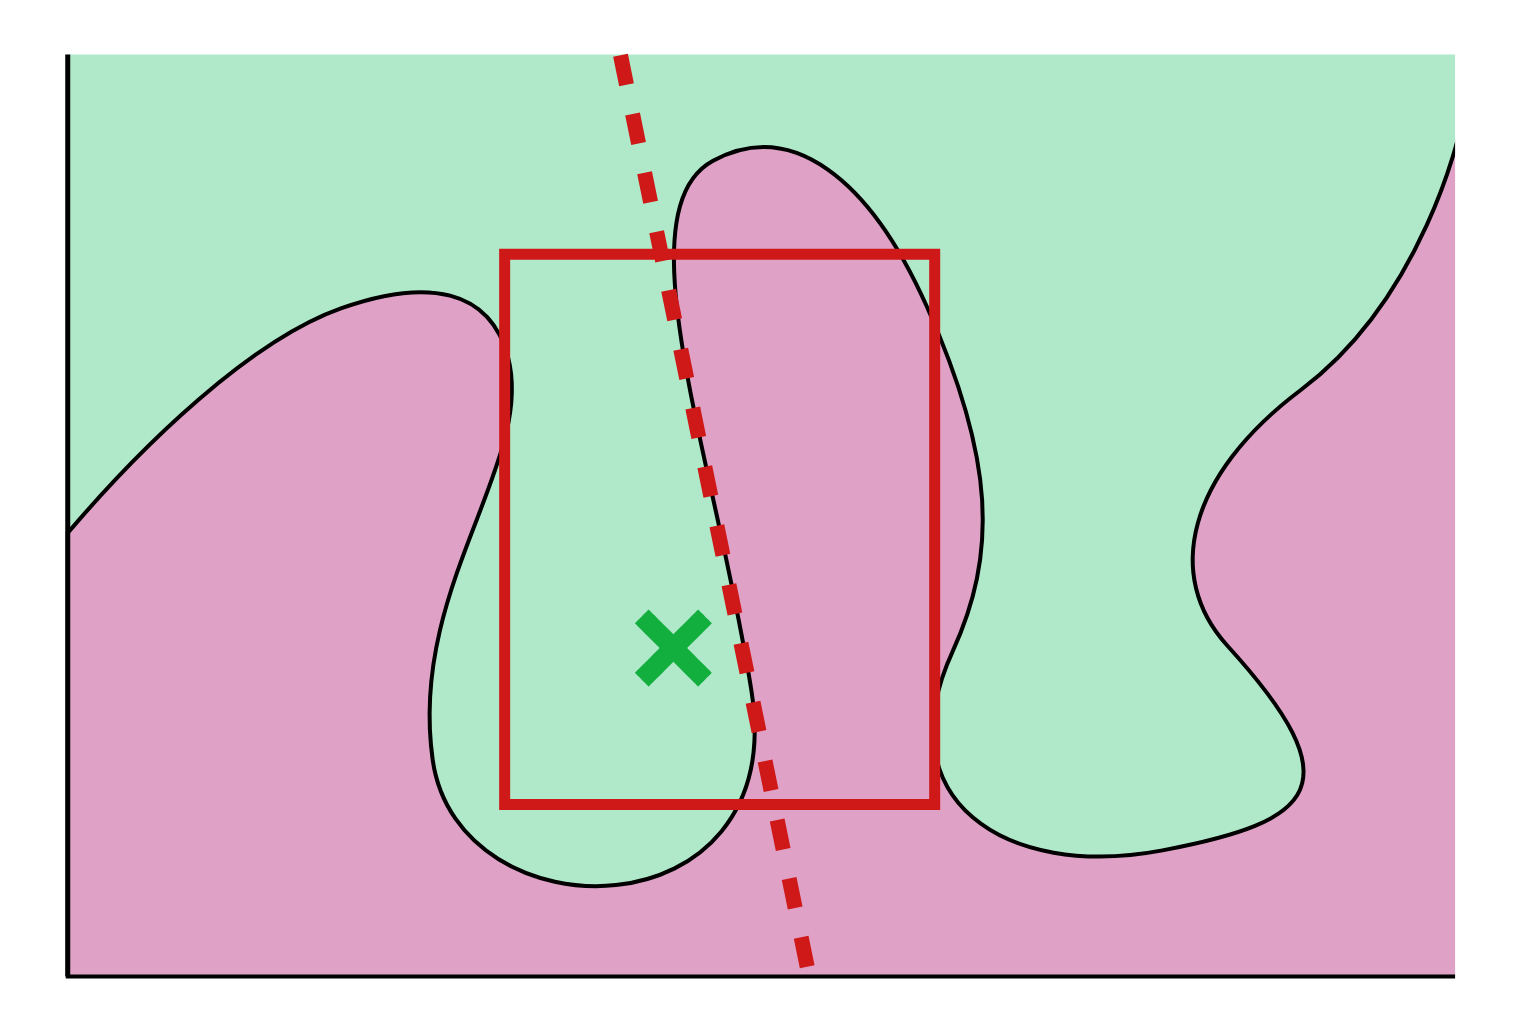
\includegraphics[width=\textwidth]{rlime3}
    \caption{%
      R-LIME:
      Maximizes coverage of a rectangular region containing the focal point
      under lower constraints on the accuracy of the linear classifier.
    }\label{fig:rlime}
  \end{subfigure}
  \caption{%
    Visual comparison of LIME, Anchor, BELLA and R-LIME (our proposed method).
    The solid line represents the rectangular region containing the focal
    point, and the dashed line represents the learned approximation model.
  }
\end{figure}

\subsection{Overview}
We propose R-LIME,
a method that aims to address the limitations of LIME \cite{ribeiro2016why},
Anchor \cite{ribeiro2018anchors} and BELLA \cite{radulovic2023bella}.
Our method locally approximates the given black-box classifier $f$
around the focal point $x$ by a linear classifier $g$ similar to LIME and BELLA,
but samples parturbation from a rectangular region similar to Anchor
(\cref{fig:rlime}).
The accuracy of $g$ is defined as the "accuracy" of the rule,
and the generality of explanations is defined as the "coverage" of the rule.

Anchor maximizes the coverage of region $A$
as long as the probability of the output of the black-box classifier $f$ matching $f(x)$
within $A$ exceeds a given threshold $\tau$.
The proposed method, on the other hand, learns an linear classifier $g$
within the rectangular region $A$ and maximizes the coverage of $A$
under lower constraints on the accuracy of $g$. 
We modify the Anchor's definition of accuracy in \cref{eq:anchor_def_prec}
as follows:
\begin{equation}
  \Prec(A)=\underset{g\in G}{\max}\ \mathbb{E}_{z\sim\mathcal{D}(z|A)}
  [\mathbbm{1}_{f(z)=g(z)}]. \label{eq:def_prec}
\end{equation}
where $G$ is the set of possible linear classifiers.
By solving the optimization problem in \cref{eq:main_problem}
under the modified accuracy definition in \cref{eq:def_prec},
we can select the rule that enables explanation with high accuracy and generality.
The characteristics of R-LIME are listed below:
\begin{itemize}
  \item The approximation region is optimal and interpretable.
  \item The dataset is not directly accessed, and only the distribution is utilized.
  \item The number of samples is dynamically determined
        based on the estimated accuracy without the need for predefining it.
\end{itemize}

\subsection{Algorithm}\label{sec:alg}
{%
  \begin{figure}[t]
    \centering
    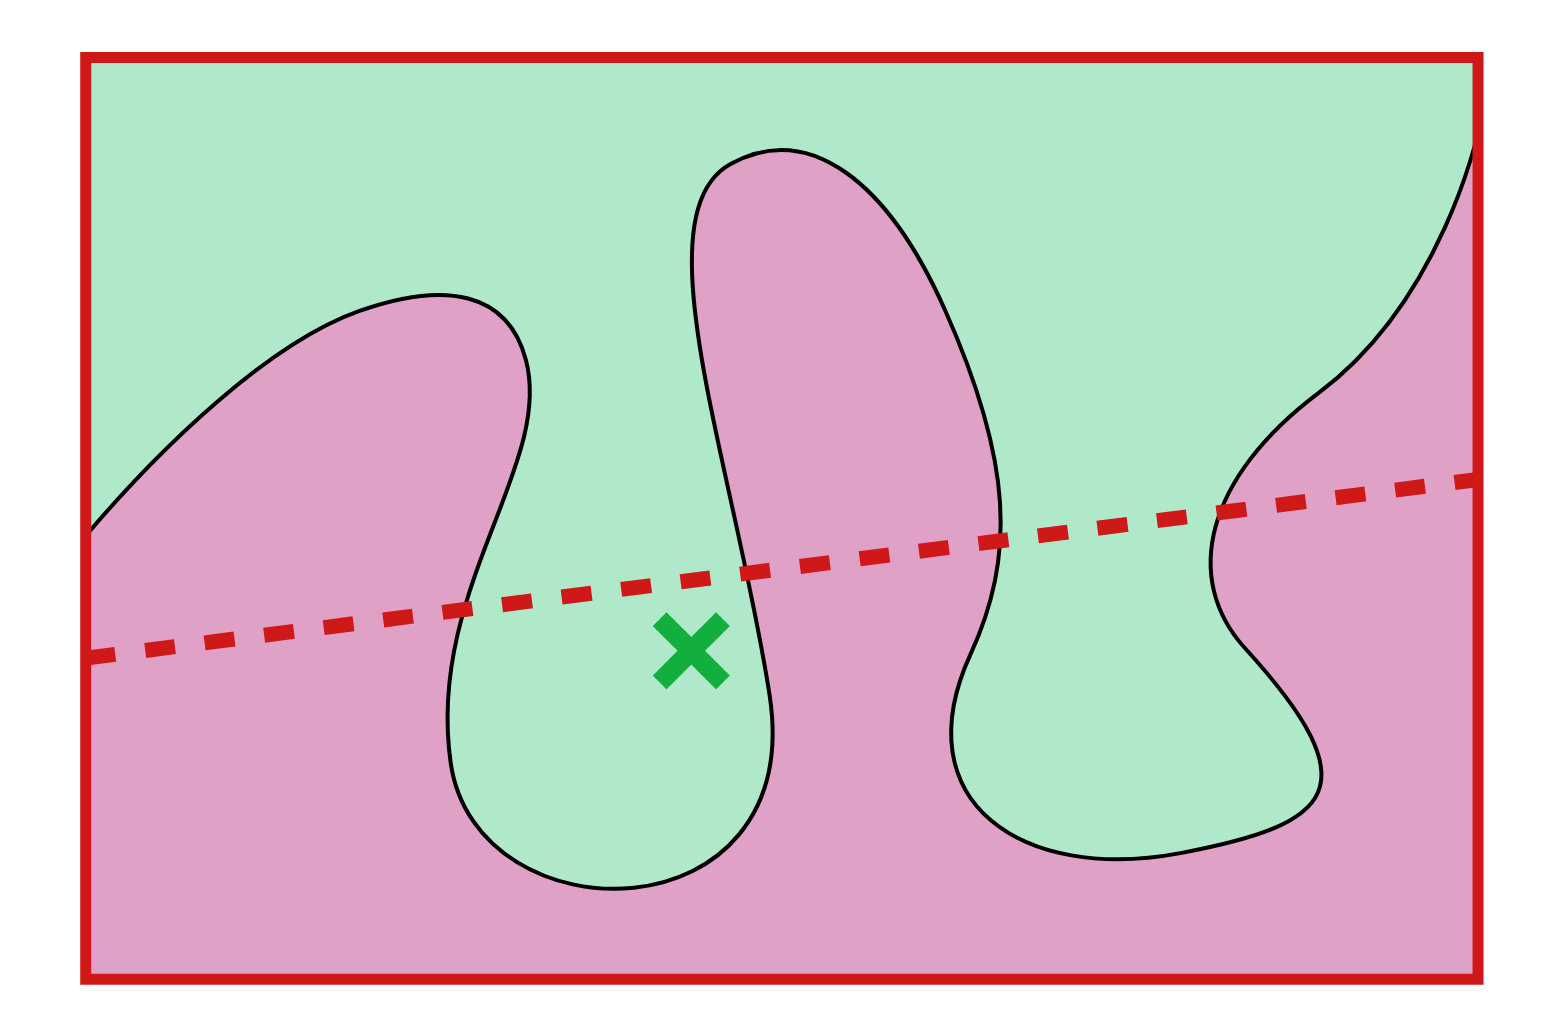
\includegraphics[width=0.32\textwidth]{rlime1}
    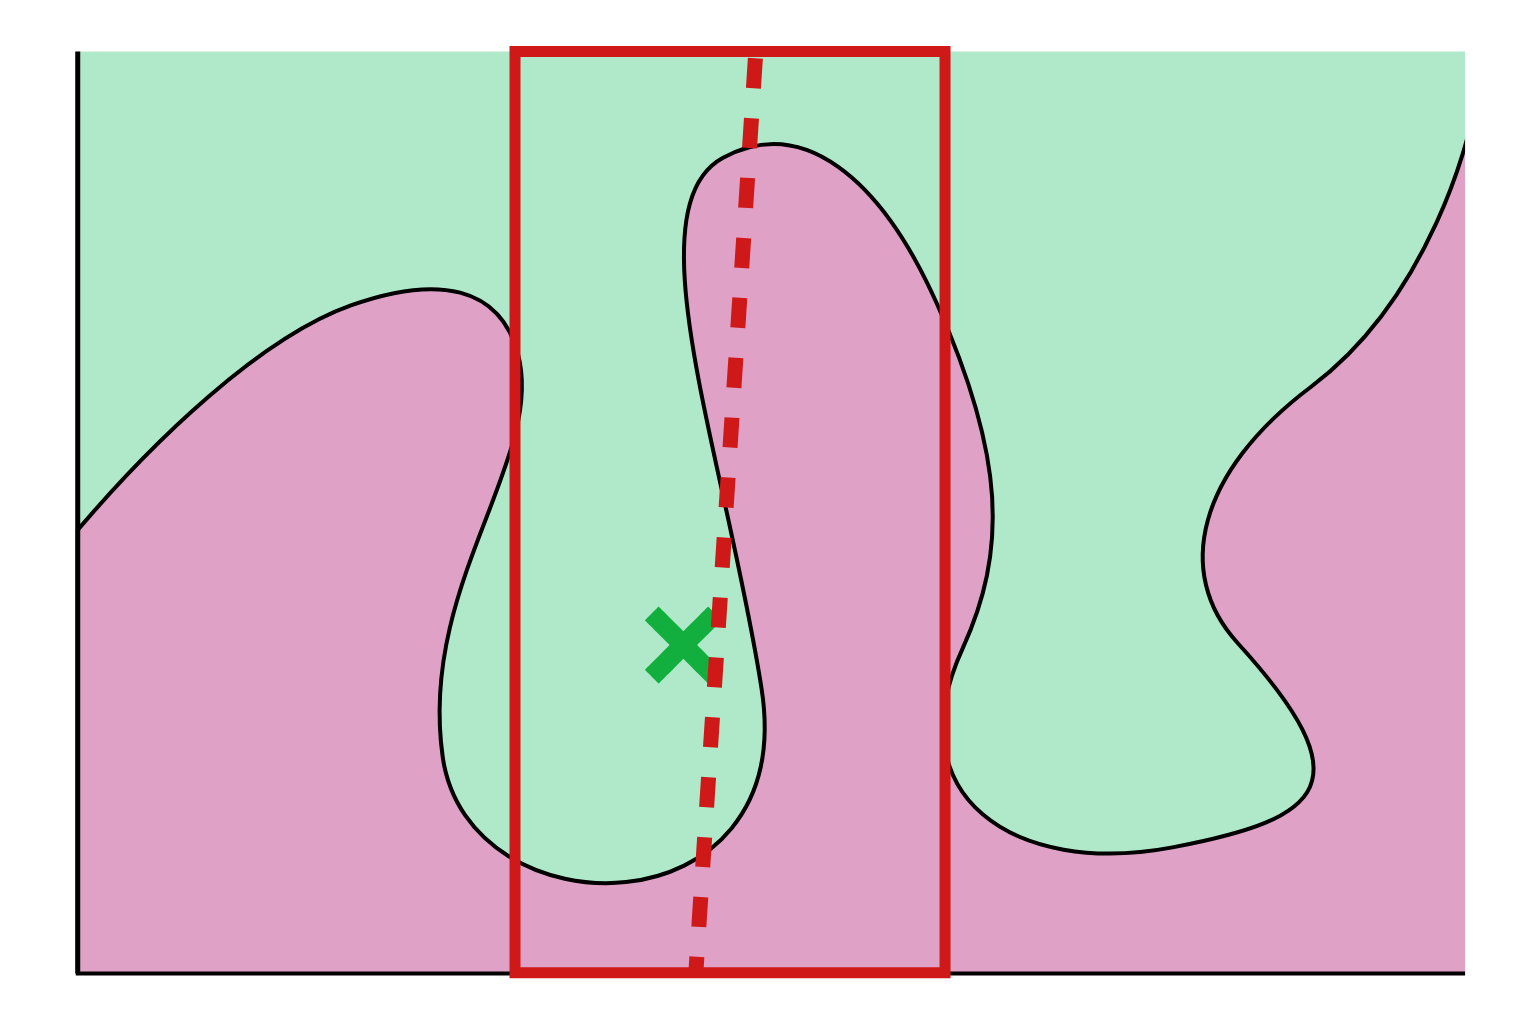
\includegraphics[width=0.32\textwidth]{rlime2}
    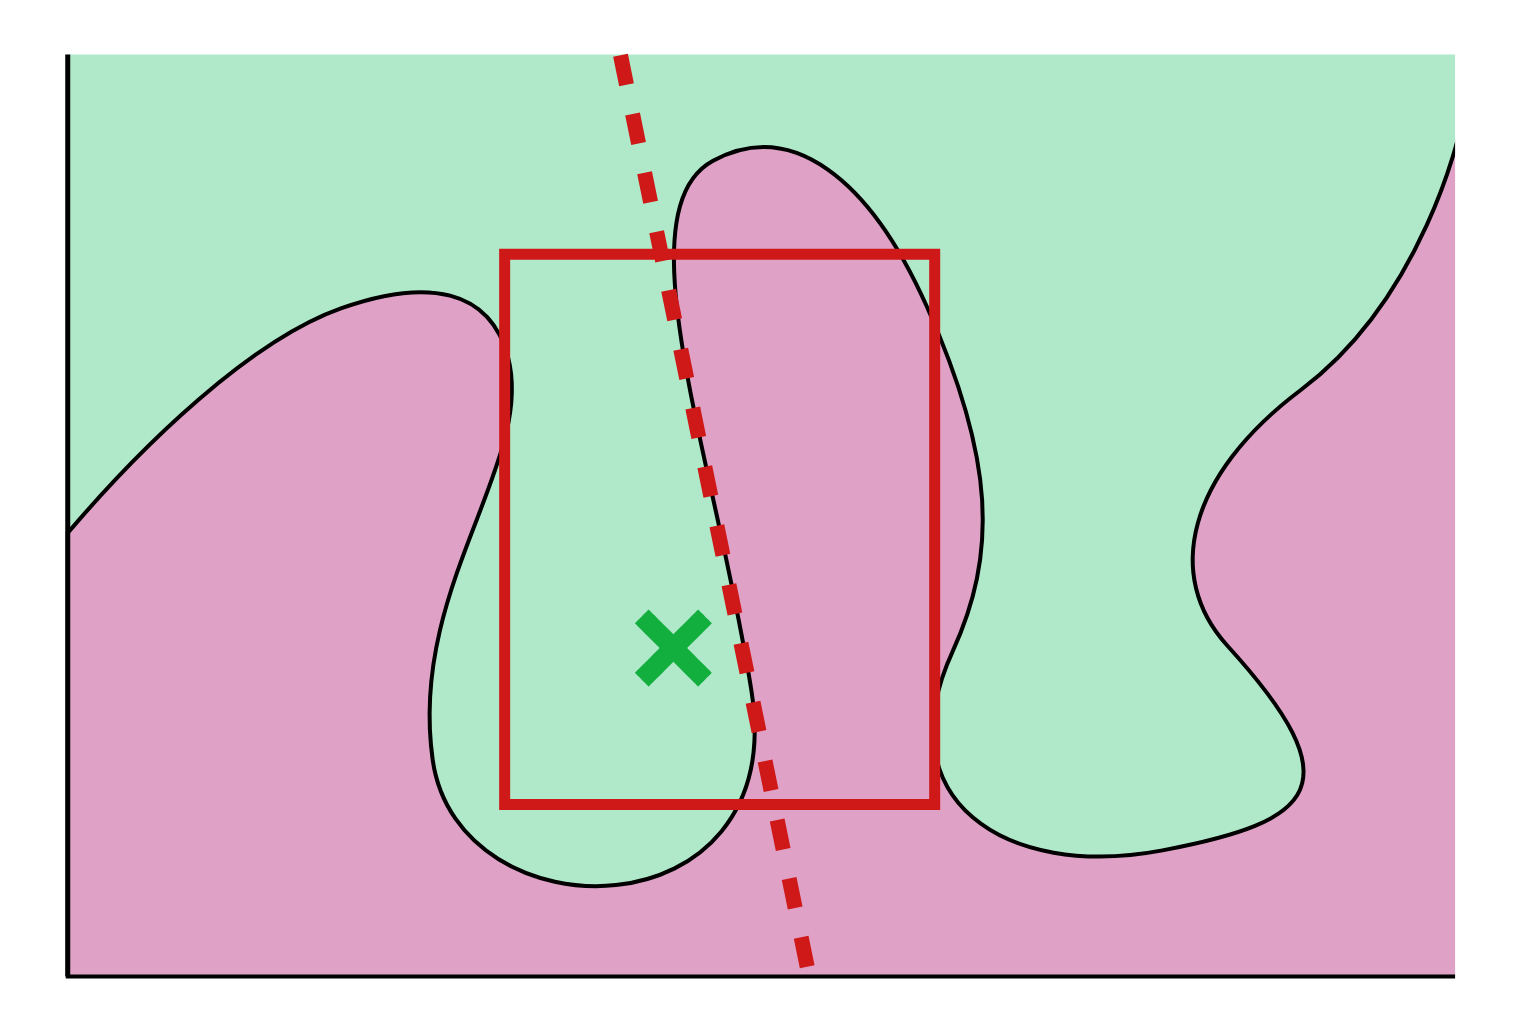
\includegraphics[width=0.32\textwidth]{rlime3}
    \caption{%
      Overview of the R-LIME algorithm.
      The progression of the algorithm is illustrated from left to right.
      The solid line represents the rectangular region $A$,
      and the dashed line represents the linear approximation model $g$
      learned within $A$.
      The initial value of $A$ is an empty rule (entire input space),
      and predicates are added to $A$, reducing coverage.
      The process continues until $\Prec(A)\ge\tau$,
      at which point the rule with the maximum coverage is output.
    }
  \end{figure}
  \begin{algorithm}[p]
    \caption{R-LIME}\label{alg:greedy-search}
\begin{algorithmic}[1]
	\Require{%
		Black-box model $f$, Target instance $x$,
		Distribution $\mathcal{D}$,
		Threshold $\tau$, Beam width $B$, Tolerance $\epsilon$,
		Confidence level $1-\delta$
	}
	\Ensure{%
		Rule $A^*$ satisfying Eq.~\eqref{eq:main-problem}
	}
	\State{$A^*\gets\textbf{null},\ \mathcal{A}_0\gets\emptyset,\ t\gets0$}
	% \Comment{%
	%   Initialize the set of candidate rules $\mathcal{A}_0$ to $\emptyset$
	% }
	\Comment{Initialize the set of candidate rules $\mathcal{A}_0$ to $\emptyset$}
	\While{$A^*=\textbf{null}$}
	\State$t\gets t+1$
	\State$\cands_t\gets$ \Call{GenerateCands}
	{$\mathcal{A}_{t-1}$}
	\State$\mathcal{A}_t\gets$ \Call{B-BestCands}
	{$\cands_{t},\mathcal{D},B,\epsilon,\delta$}
	\State$A^*\gets$ \Call{LargestCand}
	{$\mathcal{A}_t,\tau,\delta$}
	\EndWhile%
\end{algorithmic}

  \end{algorithm}
  \begin{algorithm}[p]
    \caption{Generating new candidate rules}\label{alg:generate-cands}
\begin{algorithmic}[1]
	\Function{GenerateCands}{$\mathcal{A},x$}
	\IIf{$\mathcal{A}=\emptyset$}{\Return{$\{\mathit{true}\}$}}
	\Comment{An initial empty rule always returns $\mathit{true}$}
	\State$\cands\gets\emptyset$
	\ForAll{$A\in\mathcal{A}$}
	\ForAll{$a\in (T(x)\setminus A)$}
	\State$\cands\gets\bar{\mathcal{A}}\cup(A\wedge a)$
	\Comment{Get a new rule by adding a new predicate $a$ to $A$}
	\EndFor%
	\EndFor%
	\State\Return{$\cands$}
	\EndFunction%
\end{algorithmic}

  \end{algorithm}
  \def\myidt{\hspace{\algorithmicindent}}
  \begin{algorithm}[p]
    \caption{%
	Searching rules with highest accuracy (KL-LUCB~\cite{kaufmann2013information})
}\label{alg:best-cands}
\begin{algorithmic}[1]
	\Function{B-BestCands}{$\cands,\mathcal{D},B,\epsilon,\delta$}
	\State\textbf{initialize} $\Prec,\Prec_{u},\Prec_{l}$ for $\forall A\in\cands$
	\State$\mathcal{A}\gets\Call{B-ProvisionallyBestCands}{\cands}$
	\Comment{$B$ rules with highest accuracy}
	\State$A\gets\arg\min_{A\in\mathcal{A}}\Prec_{l}(A,\delta)$
	\Comment{The rule with the smallest lower bound}
	\State$A'\gets\arg\max_{A'\notin(\cands\setminus\mathcal{A})}\Prec_{u}(A',\delta)$
	\Comment{The rule with the largest upper bound}
	\While{$~\Prec_{u}(A',\delta)-\Prec_{l}(A,\delta)>\epsilon$}
	\State\textbf{sample} $z\sim\mathcal{D}(z|A),z'\sim\mathcal{D}(z'|A')$
	\State\textbf{update} $\Prec,\Prec_{u},\Prec_{l}$ for $A$ and $A'$
	\State$\mathcal{A}\gets\Call{B-ProvisionallyBestCands}{\cands}$
	\State$A\gets\arg\min_{A\in\mathcal{A}}\Prec_{l}(A,\delta)$
	\State$A'\gets\arg\max_{A'\notin(\cands\setminus\mathcal{A})}\Prec_{u}(A',\delta)$
	\EndWhile%
	% \State\algorithmicdo%
	% \State\myidt$\mathcal{A}\gets\Call{B-ProvisionallyBestCands}{\cands}$
	% \State\myidt$A\gets\arg\min_{A\in\mathcal{A}}\Prec_{l}(A)$
	% \State\myidt$A'\gets\arg\max_{A'\notin(\cands\setminus\mathcal{A})}\Prec_{u}(A')$
	% \State\myidt\textbf{sample} $z\sim\mathcal{D}(z|A),z'\sim\mathcal{D}(z'|A')$
	% \State\myidt\textbf{update} $\Prec,\Prec_{u},\Prec_{l}$ for $A$ and $A'$
	% \State\algorithmicwhile$~\Prec_{u}(A')-\Prec_{l}(A)>\epsilon$
	\State\Return{$\mathcal{A}$}
	\EndFunction%
\end{algorithmic}

  \end{algorithm}
  \begin{algorithm}[p]
    \caption{%
  Selecting the largest rule satisfying the constraint
}\label{alg:largest_valid_cand}
\begin{algorithmic}[1]
  \Function{LargestCand}{$\mathcal{A},\tau,\delta$}
  \State$A^*\gets\textbf{null}$
  \ForAll{$A\in\mathcal{A}$ s.t. $\Prec_{l}(A,\delta)>\tau$}
  \IIf{$\Cov(A)>\Cov(A^*)$}{$A^*\gets A$}
  \EndFor%
  \State\Return{$A^*$}
  \EndFunction%
\end{algorithmic}

  \end{algorithm}
}

Our method's algorithm is mainly based on that used in Anchor.
For non-convex optimization problems like \cref{eq:main_problem},
greedy search are often used.
However,
greedy methods tend to converge to local optima, and to address this,
R-LIME utilizes beam search,
which selects multiple candidates at each iteration.
The pseudocode is shown in \cref{alg:greedy_search}.

\subsubsection{Generation of New Candidate Rules}
To generate new candidate rules,
one additional predicate is added to each of the $B$ candidate rules
selected in the previous iteration.
The pseudocode is shown in \cref{alg:generate_cands}.
$T(x)$ is the set of attribute-value pairs (predicates) that are true for $x$,
and $T(x)\setminus A$ is the set of predicates in $T(x)$ not included in rule $A$.

\subsubsection{Selection of Candidate Rules with Maximum Accuracy}
Given the set of generated candidate rules $\cands$,
the algorithm selects the top $B$ candidates with the highest accuracy.
This is treated as an optimal arm identification problem in the multi-armed bandit framework.
Each candidate rule $A_i\in\cands$ is considered an arm,
and their accuracy $\Prec(A_i)$ is treated as the distribution of rewards.
By sampling $z\sim\mathcal{D}(\cdot|A_i)$
and obtaining the reward $\mathbbm{1}_{f(z)=g_i(z)}$ for each trial,
the algorithm updates $g_i$ using the sampled perturbation vector $z$
and the pseudo-label $f(z)$ after each trial.
To efficiently select the rule (arm) with the highest accuracy,
we employ the KL-LUCB algorithm \cite{kaufmann2013information}.
The pseudocode is shown in \cref{alg:best_cands}.
For tolerance $\epsilon\in[0,1]$, the KL-LUCB algorithm guarantees below:
\begin{equation}
  P(\underset{A\in\cands}{\min}\Prec(A)\ge
  \underset{A'\in\mathcal{A}}{\min}\Prec(A')-\epsilon)\ge1-\delta.
\end{equation}
However, 
the KL-LUCB algorithm assumes that the reward distribution for each arm
remains unchanged, 
while our method updates the classifier $g_i$ with each sampling,
which may not satisfy this assumption.
This issue is discussed further in \cref{sec:reward}.

\subsubsection{Selection of the Rule with Maximum Coverage Meeting the Constraint}
To satisfy the constraint imposed by \cref{eq:const_prec}, rule $A$ needs to fulfill the lower bound constraint:
\begin{equation}
  \Prec_{l}(A,\delta)>\tau
  \label{eq:stop_condition}
\end{equation}
where $\Prec_{l}(A,\delta)$ is the lower limit of
the $100(1-\delta)$\% confidence interval for $\Prec(A)$.
If the received set of candidate rules, $\mathcal{A}$,
includes a rule satisfying \cref{eq:stop_condition},
the one with the maximum coverage among them is selected,
and the iteration is terminated.
If $\mathcal{A}$ does not contain any rule satisfying \cref{eq:stop_condition},
it returns \textbf{null},
and proceeds to the next iteration.
The pseudocode is presented in \cref{alg:largest_valid_cand}.

% The algorithmic procedure outlined above approximates
% the solution to the optimization problem in \cref{eq:main_problem}
% under the definition of accuracy in \cref{eq:def_prec}. 

\section{Experiments}
To verify the effectiveness of the proposed method,
We compare LIME and R-LIME using a real-world dataset.

\subsection{Qualitative Evaluation}
\subsubsection{Experimental Setup}\label{sec:exp_setting}
{%
  \renewcommand{\arraystretch}{1.05}
  \begin{table}[tbp]
    \centering
    \caption{%
      Attributes of the recidivism dataset used in the experiments.
      Continuous features are all discretized
      and only binary and ordinal features are considered.
    }\label{tab:rcdv}
    \begin{tabular}{llc}
      \toprule
      Attribute              & Overview                              & \# of Possible Values \\
      \midrule
      Race                   & Race (Black or White)                 & 2                     \\
      Alcohol                & Presence of serious alcohol issues    & 2                     \\
      Junky                  & Drug usage                            & 2                     \\
      Supervised Release     & Supervised release                    & 2                     \\
      Married                & Marital status                        & 2                     \\
      Felony                 & Felony or not                         & 2                     \\
      WorkRelease            & Participation in work release program & 2                     \\
      Crime against Property & Crime against property or not         & 2                     \\
      Crime against Person   & Crime against a person or not         & 2                     \\
      Gender                 & Gender (Female or Male)               & 2                     \\
      Priors                 & Number of prior offenses              & 4                     \\
      YearsSchool            & Years of formal education completed   & 4                     \\
      PrisonViolations       & Number of prison rule violations      & 3                     \\
      Age                    & Age                                   & 4                     \\
      MonthsServed           & Months served in prison               & 4                     \\
      \midrule
      Recidivism             & Recidivism or not                     & 2                     \\
      \bottomrule
    \end{tabular}
  \end{table}
}

The experiments utilized the recidivism dataset \cite{schmidt1988predicting}.
This dataset contains information on 9,549 prisoners released from
North Carolina prisons between July 1, 1979, and June 30, 1980.
The dataset includes 19 items such as race, gender,
presence of alcohol dependence, number of prior offenses, and recidivism.
For this experiment, 
we treated the binary classification problem of predicting
the presence or absence of recidivism (Recidivism) as the target label. 
We discretized continuous features and removed missing values,
resulting in 15 features. 
This problem setting can be considered as a case
where a machine learning model is introduced to decide parole for prisoners.
Since such decisions can have a significant impact on a person's life,
it is crucial for users to interpret the outputs of black-box models appropriately.

The dataset, after removing missing values,
was split into training data (7,639 instances) and test data (955 instances).
A random forest model with 50 trees was trained using the training data.
Subsequently, LIME and R-LIME explanations were generated
for two instances extracted from the test data (\cref{fig:instance}).
In R-LIME, logistic regression was used as the linear approximation model, 
and the distribution $\mathcal{D}$ was a multivariate normal distribution
estimated from the training data.
The beam width was set to $B=10$,
the confidence coefficient to $1-\delta=0.95$,
and the tolerance of the KL-LUCB algorithm to $\epsilon=0.05$.
Accuracy thresholds $\tau$ were set to $\tau=0.70,0.80,0.90$.

  {%
    
    \def\dir{python/exp1}
    \def\Asample{0012}
    \def\Bsample{0011}
    \def\index#1{\ifnum#1=0 \Asample \else \Bsample \fi}
    
    {%
      \def\AB#1{\ifnum#1=0 A\else B\fi}
      \def\mylabel#1{\ifnum#1=0 \label{fig:A-instance}\else \label{fig:B-instance}\fi}
      \renewcommand{\arraystretch}{1.02}
      \begin{figure}[tbp]
        \foreach\a in {0,1}{%
            \centering
            \begin{subfigure}{\textwidth}
              \centering
              \begin{tabular}{p{14em}m{16em}}
                \toprule
                \csvreader[no head, late after line= \\]{%
                  \dir/\index{\a}.csv
                }{}{%
                \ifnum\thecsvrow=16 \midrule\fi\csvcoli & \csvcolii
                }
                \bottomrule
              \end{tabular}
              \caption{Instance~\AB{\a}}\mylabel{\a}
              \vspace{15pt}
            \end{subfigure}
          }
        \vspace{-15pt}
        \caption{Two instances sampled from recidivism dataset.}\label{fig:instance}
      \end{figure}
    }
    {%
      \def\scale{0.315}
      \def\imgwidth{0.495\textwidth}
      \def\hspacebase{\hspace{-1.5em}}
      \def\vspacebase{\vspace{0.5em}}
      \def\vspacebeforecaption{\vspace{-0.4em}}
      \begin{figure}[p]
        \centering
        \begin{subfigure}[t]{\imgwidth}
          \hspacebase
          \includegraphics[scale=\scale]{\dir/lime-\Asample}
          \vspacebeforecaption
          \caption{LIME}\label{fig:A-lime}
          \vspacebase
        \end{subfigure}
        \begin{subfigure}[t]{\imgwidth}
          \hspacebase
          \hspace{1.0em}
          \includegraphics[scale=\scale]{\dir/newlime-\Asample-70}
          \vspacebeforecaption
          \caption{R-LIME ($\tau=0.70$)}\label{fig:A-rlime-70}
          \vspacebase
        \end{subfigure}
        \begin{subfigure}[t]{\imgwidth}
          \hspacebase
          \includegraphics[scale=\scale]{\dir/newlime-\Asample-80}
          \vspacebeforecaption
          \caption{R-LIME ($\tau=0.80$)}\label{fig:A-rlime-80}
        \end{subfigure}
        \begin{subfigure}[t]{\imgwidth}
          \hspacebase
          \includegraphics[scale=\scale]{\dir/newlime-\Asample-90}
          \vspacebeforecaption
          \caption{R-LIME ($\tau=0.90$)}\label{fig:A-rlime-90}
        \end{subfigure}
        \caption{Explanation for Instance A by LIME and R-LIME.}\label{fig:A}
      \end{figure}
      \begin{figure}[p]
        \centering
        \begin{subfigure}[t]{\imgwidth}
          \hspacebase
          \includegraphics[scale=\scale]{\dir/lime-\Bsample}
          \vspacebeforecaption
          \caption{LIME}\label{fig:B-lime}
          \vspacebase
        \end{subfigure}
        \begin{subfigure}[t]{\imgwidth}
          \hspacebase
          \includegraphics[scale=\scale]{\dir/newlime-\Bsample-70}
          \vspacebeforecaption
          \caption{R-LIME ($\tau=0.70$)}\label{fig:B-rlime-70}
          \vspacebase
        \end{subfigure}
        \begin{subfigure}[t]{\imgwidth}
          \hspacebase
          \includegraphics[scale=\scale]{\dir/newlime-\Bsample-80}
          \vspacebeforecaption
          \caption{R-LIME ($\tau=0.80$)}\label{fig:B-rlime-80}
        \end{subfigure}
        \begin{subfigure}[t]{\imgwidth}
          \hspacebase
          \hspace{0em}
          \includegraphics[scale=\scale]{\dir/newlime-\Bsample-90}
          \vspacebeforecaption
          \caption{R-LIME ($\tau=0.90$)}\label{fig:B-rlime-90}
        \end{subfigure}
        \caption{Explanation for Instance B by LIME and R-LIME}\label{fig:B}
      \end{figure}
    }
  }
\subsubsection{Experimental Results}
The results of the experiment are shown in \cref{fig:A,fig:B}.
The values assigned to each attribute name represent the contribution
(weights of the learned linear classifier)
to the output of the black-box classifier,
normalized such that the absolute sum is 1.
The figures also display the 5 attributes with the highest absolute contribution.

Explanations generated by LIME (\cref{fig:A-lime,fig:B-lime}) indicate that
attributes such as having a significant prior record (Prior) or committing a
crime against property (Crime against Property) primarily contribute positively
to the prediction (predicting that the prisoner will be re-arrested).
On the other hand,
attributes like older age (Age), being married (Married),
and being of white race (Race) contribute negatively to the prediction
(predicting that the prisoner will not be re-arrested).
While these LIME explanations provide valuable insights into the behavior of
the black-box model,
they do not explicitly indicate the application scope of the explanations, 
leaving users unable to determine to which inmates the explanations are applicable.

In contrast, R-LIME expresses the application scope of explanations
as a conjunction of predicates.
For example, the explanation for instance A
under $\tau=0.70$ (\cref{fig:A-rlime-70}) indicates that it is applicable
only to married prisoner (Married$=$Yes).
Furthermore, the generated explanations include the accuracy and coverage of
the approximation region, allowing users to evaluate how reliable the
explanations are.
For example, the coverage of the explanation for instance B under $\tau=0.90$
(\cref{fig:B-rlime-90}) is 0.002,
indicating that the decision boundaries around instance B are complex,
making it challenging to obtain a high-accuracy linear approximation.
This allows users to discern that the application scope of this explanation is
very narrow, limiting its utility.

\subsection{Quantitative Evaluation}\label{sec:exp2}
\subsubsection{Experimental Setup}
To demonstrate that R-LIME learns a highly accurate linear approximation model
in the optimized approximation region,
we conducted a comparison of the local accuracy of explanations
between LIME and R-LIME.
Using the same settings as in \cref{sec:exp_setting},
we randomly sampled 100 instances from the test data of the recidivism dataset
and generated explanations (with $\tau=0.70,0.80,0.90$) using LIME and R-LIME.
We then sampled 10,000 instances within the rectangular region
obtained by R-LIME and calculated the local accuracy of both methods.
\subsubsection{Experimental Results}
\begin{figure}[tbp]
  \centering
  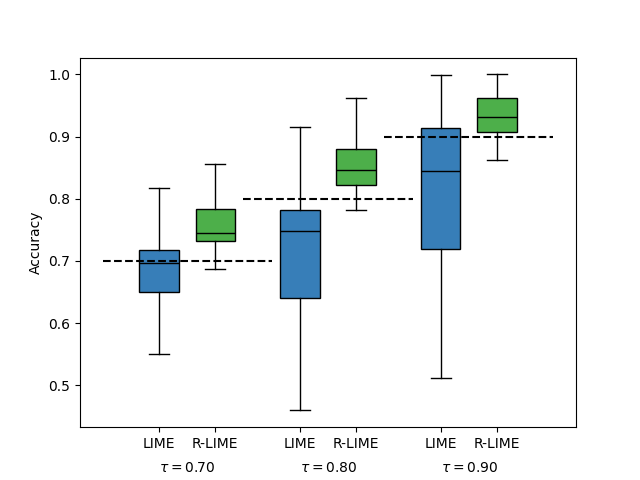
\includegraphics[width=0.55\textwidth]{python/exp2/box_plot}
  \caption[Comparison of Local Accuracy between R-LIME and LIME]{%
    Comparison of local accuracy between LIME and R-LIME.
    R-LIME achieved higher and less variable accuracy compared to LIME
    for all values of $\tau$.
  }\label{fig:box_plot}
\end{figure}
The results are presented in \cref{fig:box_plot},
showcasing the distribution of the accuracy of the linear approximation models
learned by LIME and R-LIME.
R-LIME exhibits higher accuracy compared to LIME for all values of $\tau$.
This suggests that the linear classifiers learned by LIME and R-LIME
differ significantly,
and R-LIME learns a high-accuracy linear classifier adapted to the rectangular region.
Additionally, as $\tau$ increases,
the variability in the accuracy of LIME widens.
This indicates that the linear classifiers learned by LIME may not function
effectively as approximation models depending on how the region is selected.

\section{Challenges and Future Perspectives}
 {%
  \def\imgwidth{0.49\textwidth}
  \begin{figure}[t]
    \centering
    \begin{subfigure}[t]{\imgwidth}
      \centering
      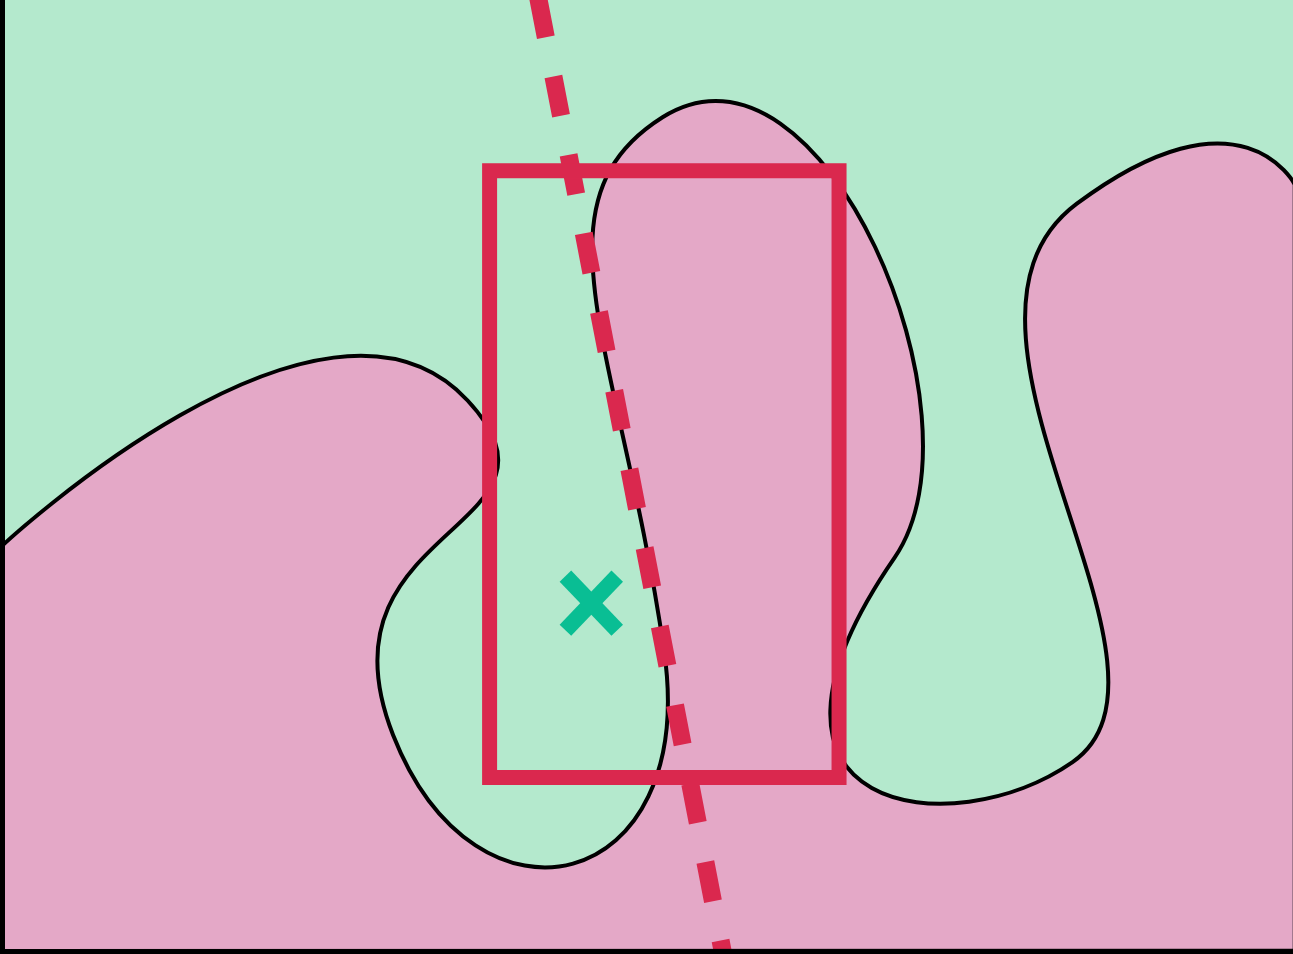
\includegraphics[width=0.78\textwidth]{newlime}
      \caption{R-LIME for balanced data.}\label{fig:balanced}
    \end{subfigure}
    \begin{subfigure}[t]{\imgwidth}
      \centering
      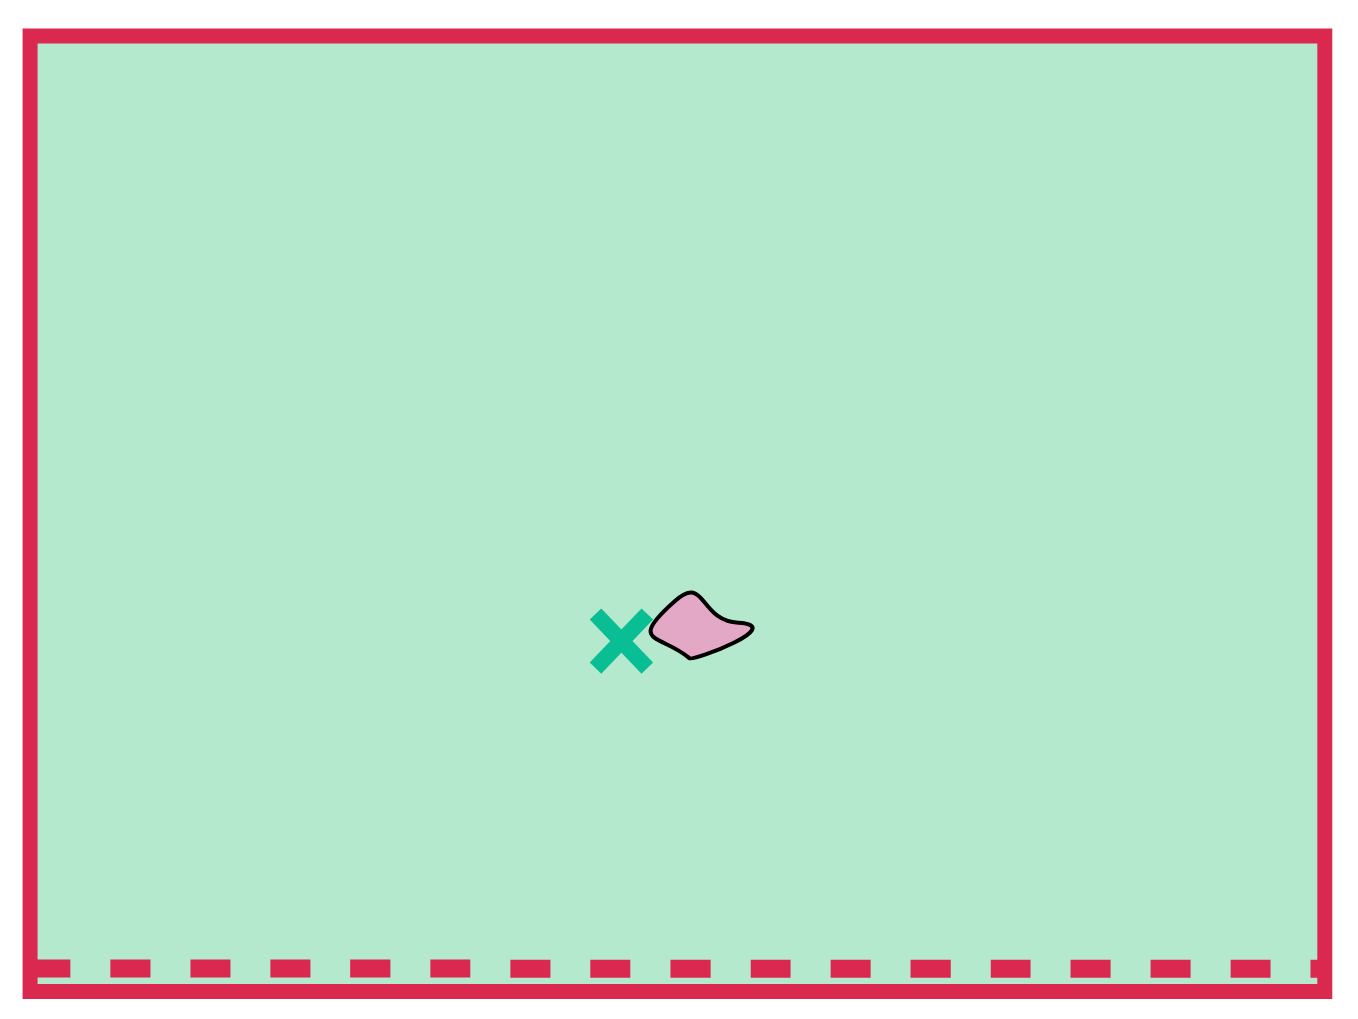
\includegraphics[width=0.8\textwidth]{newlime_for_imbalanced_data}
      \caption{R-LIME for imbalanced data.
      }\label{fig:imbalanced}
    \end{subfigure}
    \caption{%
      Behavior of R-LIME for balanced and imbalanced data.
      In case of imbalanced label distribution,
      the approximation region covers the entire input space and the
      linear approximation model always outputs the majority label.
    }
    \vspace{10pt}
  \end{figure}
 }

\subsection{Behavior Regarding Imbalanced Label Distribution}
R-LIME may generate less useful explanations
when there is bias in the distribution of black-box model outputs.
When the distribution of black-box model outputs is significantly biased
for a given accuracy threshold $\tau$
(when the ratio of the minority label is less than $1-\tau$),
the approximation region generated by R-LIME covers the entire input space,
and the learned linear classifier always outputs the majority label
(\cref{fig:imbalanced}).

A first possible solution to this problem is modifying the loss function.
Using weighted logistic loss or Focal Loss \cite{lin2020focal}
as the loss function might lead to the generation of more useful explanations
in the case of imbalanced label distribution.
Another solution involves adding constraints
to limit the label distribution bias within the approximation region.
In addition to \cref{eq:const_prec}, adding a constraint like
\begin{equation}
  {\left(\mathbb{E}_{z\sim\mathcal{D}(z\mid A)}[\mathbbm{1}_{f(z)=1}]-\frac{1}{2}\right)}^2<\mu
\end{equation}
could suppress the excessive expansion of the approximation region.

\subsection{Changes in Reward Distribution in Optimal Arm Identification}\label{sec:reward}
{%
  \renewcommand{\arraystretch}{1.1}
  \begin{table}[tbp]
    \centering
    \caption{%
      Deviation between the estimated accuracy and the true accuracy.
      Deviation was relatively small considering confidence level $1-\delta=0.95$.
    }\label{tab:reward}
    \begin{tabular}{cccc}
  \toprule
                     & Estimated acc. & True acc. & Deviation \\
  \midrule
  Average            & .811           & .829      & .012      \\
  Standard Deviation & .018           & .023      & .017      \\
  \bottomrule
\end{tabular}

  \end{table}
}
In R-LIME,
the problem of selecting the rule with the highest accuracy is formulated
as the optimal arm identification problem in multi-armed bandit theory,
solved using the KL-LUCB algorithm \cite{kaufmann2013information}.
However, this algorithm assumes that the reward distribution remains constant,
while in R-LIME,
the reward distribution (accuracy of the linear approximation)
changes with every update of the approximation model after sampling.
Therefore, rewards obtained at an early stage
might influence the estimated value and deviate from the true value.

We conducted an experiment to evaluate the deviation
between the estimated accuracy and the true accuracy.
We generated explanations for 3,200 data instances sampled from the dataset,
and compared the estimated accuracy with the true accuracy.
The true accuracy was calculated based on 1,000 instances sampled
within the approximation region.
The results in \cref{tab:reward} show a mean deviation of 0.012
with a standard deviation of 0.017.
While the deviation was relatively small considering confidence level $1-\delta=0.95$,
we should modify the selection algorithm to consider the varying accuracy.

\subsection{Evaluation through User Studies}
Given the nature of the field of "interpretable machine learning,"
where the goal is to "interpret" machine learning models,
it is challenging to quantitatively compare various methods.
While quantitative experiments were conducted in \cref{sec:exp2},
they mainly demonstrated that the proposed method generates
locally accurate explanations compared to LIME.
The results do not directly prove the high interpretability of the proposed method.

One potential method to quantitatively evaluate "interpretability" is
through user studies.
For example, \cite{ribeiro2018anchors} conducted user studies,
assuming that if users could predict the output of a black-box model
with high accuracy based on provided explanations,
those explanations contained valuable information about the model's behavior.
Similarly,
conducting user studies in this research would be desirable
to evaluate the interpretability of the proposed method.

\section{Conclusion}
We identified challenges in existing methods for local model-agnostic post-hoc
explanations of black-box classifiers and proposed R-LIME to address them.
We represented the rectangular region for local linear approximation as a
conjunction of feature predicates and proposed an algorithm to
maximize coverage under the constraint of minimum approximation accuracy.
Comparing the outputs of LIME and R-LIME on real-world datasets,
we demonstrated that explanations provided by R-LIME have clearer application
scopes and can be evaluated by users for reliability and generality.
However, we discussed the instability of behavior concerning imbalanced label
distributions and raised questions about the theoretical validity of using
the KL-LUCB algorithm.

\subsubsection{Acknowledgements}
% Please place your acknowledgments at
% the end of the paper, preceded by an unnumbered run-in heading (i.e.
% 3rd-level heading).
I would like to express my gratitude to Associate Professor Keigo Kimura
from the Department of Mathematical Science,
Division of Information Recognition,
Graduate School of Information Science and Technology, Hokkaido University.
He provided invaluable guidance,
from setting the research theme to outlining the strategy and content of this study.
Additionally,
I appreciate the diverse insights shared by Professor Mineichi Kudo in the same laboratory.
Finally, I am deeply thankful to all the members of the laboratory
for their helpful advice and collaboration throughout the research process.

%
% ---- Bibliography ----
%
% BibTeX users should specify bibliography style 'splncs04'.
% References will then be sorted and formatted in the correct style.
%
\bibliographystyle{splncs04}
\bibliography{MyRef/ref}
%
\end{document}
